%===============================================================================
% Test Report
%===============================================================================
% $Id: test-report.tex 248 2005-01-30 23:25:27Z thom $
%===============================================================================


%===============================================================================
% Configuration
%===============================================================================


%-------------------------------------------------------------------------------
% \documentclass and \usepackage directives
%-------------------------------------------------------------------------------
\documentclass[a4paper,fleqn,titlepage]{article} 
%\usepackage{ngerman}
\usepackage[latin1]{inputenc}
\usepackage[T1]{fontenc}
\usepackage[small,hang,bf]{caption2}
\usepackage{fancyhdr}
\usepackage[nice]{nicefrac}
\usepackage{color,listings}
\usepackage{alltt}


% Compilation with latex or pdflatex?
\newif\ifpdf 
\ifx\pdfoutput\undefined 
  \pdffalse
\else
  \pdfoutput=1 
  \pdftrue 
\fi 

% Compilation with pdflatex
\ifpdf
 
  \usepackage[pdftex]{graphicx}

  \usepackage[
    pdftex,
    a4paper,
    bookmarks,
    pdfstartview=FitH,    % starts with page width
    bookmarksopen,        % opens index
    bookmarksnumbered,    % index with numbering
    colorlinks,           % links with color, otherwise with border
    linkcolor=blue,       % Standard red
    citecolor=blue,       % Standard green
    urlcolor=magenta,     % Standard cyan
    filecolor=blue
  ]{hyperref} 

  \pdfinfo{
    /Title      (Test Report)
    /Author     (Thomas Weibel, Martin Luder, Michael K�ser)
    /Subject    (Eiffel programming)
    /Keywords   (Programming, EiffelRSS)
  }

  % Use default Acrobat reader fonts
  \usepackage{mathpazo}

  % Use CM fonts (increases document size)
  % \usepackage{ae}

% Compilation with latex
\else 

  \usepackage{graphicx} 

\fi


%-------------------------------------------------------------------------------
% Configure \maketitle
%-------------------------------------------------------------------------------
\title{EiffelRSS \\ Test Report}
\author{
  Michael K\"aser <kaeserm@student.ethz.ch>
  \and 
  Martin Luder <luderm@student.ethz.ch>
  \and 
  Thomas Weibel <weibelt@student.ethz.ch>
}
\date{\today}


%-------------------------------------------------------------------------------
% Configure fancyhdr
%-------------------------------------------------------------------------------
\pagestyle{fancy}

\renewcommand{\headrulewidth}{0.1 pt}
\renewcommand{\footrulewidth}{0.1 pt}

\fancypagestyle{plain}{
  \lhead{\nouppercase{\leftmark}}
  \chead{}
  \rhead{\thepage}
  \lfoot{EiffelRSS}
  \cfoot{}
  \rfoot{Test Report}
}

\lhead{\nouppercase{\leftmark}}
\chead{}
\rhead{\thepage}

\lfoot{EiffelRSS}
\cfoot{}
\rfoot{Test Report}


%-------------------------------------------------------------------------------
% Configure listings
%-------------------------------------------------------------------------------
\lstset{showstringspaces=false,
  breaklines=true,
  breakindent=0pt,
  prebreak=\mbox{\tiny$\searrow$},
  postbreak=\mbox{{\color{blue}\tiny$\rightarrow$}},
  frame=trBL,
  framerule=0.75pt,
  framesep=4pt,
  rulesep=0.75pt
}


%-------------------------------------------------------------------------------
% Common configuration
%-------------------------------------------------------------------------------
\setlength{\parindent}{0em}
\setlength{\parskip}{1.5ex plus0.5ex minus0.5ex}
\sloppy
\setlength{\mathindent}{0em}


%-------------------------------------------------------------------------------
% Commandos
%-------------------------------------------------------------------------------
\newcommand{\hr}{\rule{\textwidth}{1pt}}


%===============================================================================
% Document
%===============================================================================
\begin{document}

\begin{titlepage}
  \newlength{\centeroffset}
  \setlength{\centeroffset}{-0.5\oddsidemargin}
  \addtolength{\centeroffset}{0.5\evensidemargin}

  \thispagestyle{empty}

  \noindent
\includegraphics[width=\textwidth]{../figures/big_ETH}\\[-3mm]
  \hr

  \vspace*{\stretch{1}}

  \makebox[0pt][l]{
    \begin{minipage}{\textwidth}
      \flushright{
        \Huge\bfseries EiffelRSS
      }

      \noindent\rule{\textwidth}{3pt}\\[2.5ex]

      \hfill\emph{
        \Large Test Report
      }
    \end{minipage}
  }

  \vspace{\stretch{1}}

  \makebox[0pt][l]{
    \begin{minipage}{\textwidth}
      \flushright{
        \bfseries 
        Michael K\"aser <kaeserm@student.ethz.ch>\\[0.3ex]
        Martin Luder <luderm@student.ethz.ch>\\[0.3ex]
        Thomas Weibel <weibelt@student.ethz.ch>\\[0.3ex]
      }
    \end{minipage}
  }

  \vspace{\stretch{1}}

  \noindent\hr\\[1mm]
  
\includegraphics[width=\textwidth]{../figures/big_inf}
\end{titlepage}

% Use roman page numbering
\pagenumbering{roman}

\begin{abstract}
  This document describes the testing framework of EiffelRSS and how
  Newsreader was tested.
\end{abstract}

\section{Library}
\label{sec:library}

% Set page counter to zero
\setcounter{page}{0} 

% Use arabic page numbering
\pagenumbering{arabic}

EiffelRSS provides a fully automatic testing framework to test its
library.

This framework is based on Gobo Eiffel Test (getest)
\footnote{http://www.gobosoft.com/eiffel/gobo/getest/index.html} and
Gobo Eiffel ANT (geant)
\footnote{http://www.gobosoft.com/eiffel/gobo/geant/introduction.html}.

Figure \ref{fig:properties-test} shows the results of the test for
\texttt{PROPERTIES}.

\begin{figure}[htbp]
  \centering
  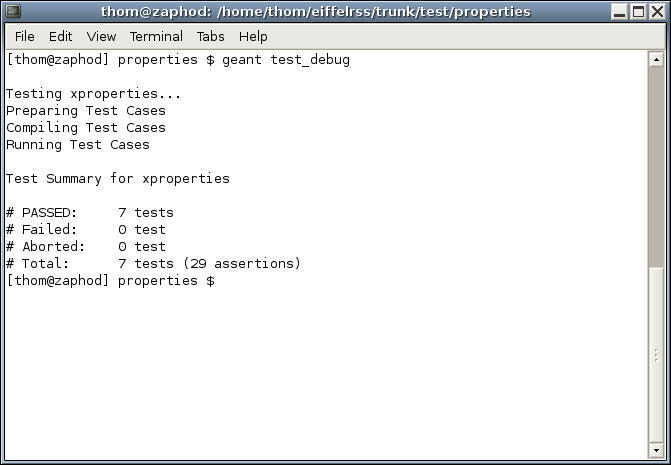
\includegraphics[width=0.7\textwidth]{./figures/properties-test}
  \caption{Screenshot of the results of the test for \texttt{PROPERTIES}}
  \label{fig:properties-test}
\end{figure}

There are more than 50 tests with more than 300 assertions implemented with an
overall line count of more than 1800 lines.

The testing framework is extremely useful when refactoring the
library. It also helped to find some bugs, eg. a nasty portability bug
in \texttt{PROPERTIES} which had to do with different line ending
characters in Unix and Windows.


\section{Newsreader}
\label{sec:newsreader}

Newsreader is an interactive application which can't be tested with an
automated testing framework.

To test Newsreader, we tried to simulate a ``normal'' user and did
lots of manual tests.

\end{document}
